\section{Introducción Conceptual---Transformers y Atención para Principiantes}
\label{sec:annex-tutorial}

Este apéndice es la rampa de entrada al artículo: explica qué es un transformer y cómo funciona la atención, para lectores sin conocimientos previos de aprendizaje profundo. Cada mecanismo se introduce mediante una analogía del mundo real y --- este es el objetivo del apéndice --- la \emph{misma} analogía regresa cada vez que el mecanismo regresa, de modo que una sola imagen mental te lleva de la primera intuición hasta las matemáticas. La Tabla~\ref{tab:tut-analogies} presenta el reparto; el ejemplo recurrente es siempre la misma oración: ``El gato come pescado''.

\begin{table}[H]
\centering
\small
\begin{tabular}{@{}lll@{}}
\toprule
\textbf{Mecanismo} & \textbf{Analogía reutilizada} & \textbf{Se introduce en}\\
\midrule
Atención & escuchar una voz en una habitación ruidosa & \S\ref{subsec:tut-attention}\\
Consultas, claves, valores & visitante, ficha de catálogo y libro en una biblioteca & \S\ref{subsec:tut-math}\\
Cabezas de atención & un equipo de analistas, una pregunta cada uno & \S\ref{subsec:tut-heads}\\
Capas apiladas & editar un ensayo en pasadas sucesivas & \S\ref{subsec:tut-layers}\\
\bottomrule
\end{tabular}
\caption{El reparto de analogías de este tutorial. Cada fila se introduce una vez y luego se reutiliza tal cual en todas las secciones posteriores, incluidas las conclusiones.}
\label{tab:tut-analogies}
\end{table}

\subsection{¿Qué es un Transformer? Palabras en Contexto}
\label{subsec:tut-context}

Un transformer es una arquitectura neuronal que procesa texto (o cualquier secuencia) interpretando el significado de cada palabra \emph{a la luz de todas las que la rodean}. El problema que resuelve se ve mejor con una palabra ambigua. Lee esto:

\begin{center}
\textit{``El banco estaba lleno de gente esperando. María fue al banco.''}
\end{center}

¿Qué significa ``banco'' en cada caso? Sola, la palabra tiene tres significados sin relación: una institución financiera, un asiento para sentarse, la orilla de un río. Dentro de la primera oración, los vecinos (``lleno de gente esperando'') votan por la sucursal. Dentro de la segunda, ``María fue al\ldots'' deja dos lecturas vivas --- podía ir a la ventanilla o al río. La Figura~\ref{fig:tut-context} contrasta las dos situaciones.

\begin{figure}[H]
\centering
\fitfigure{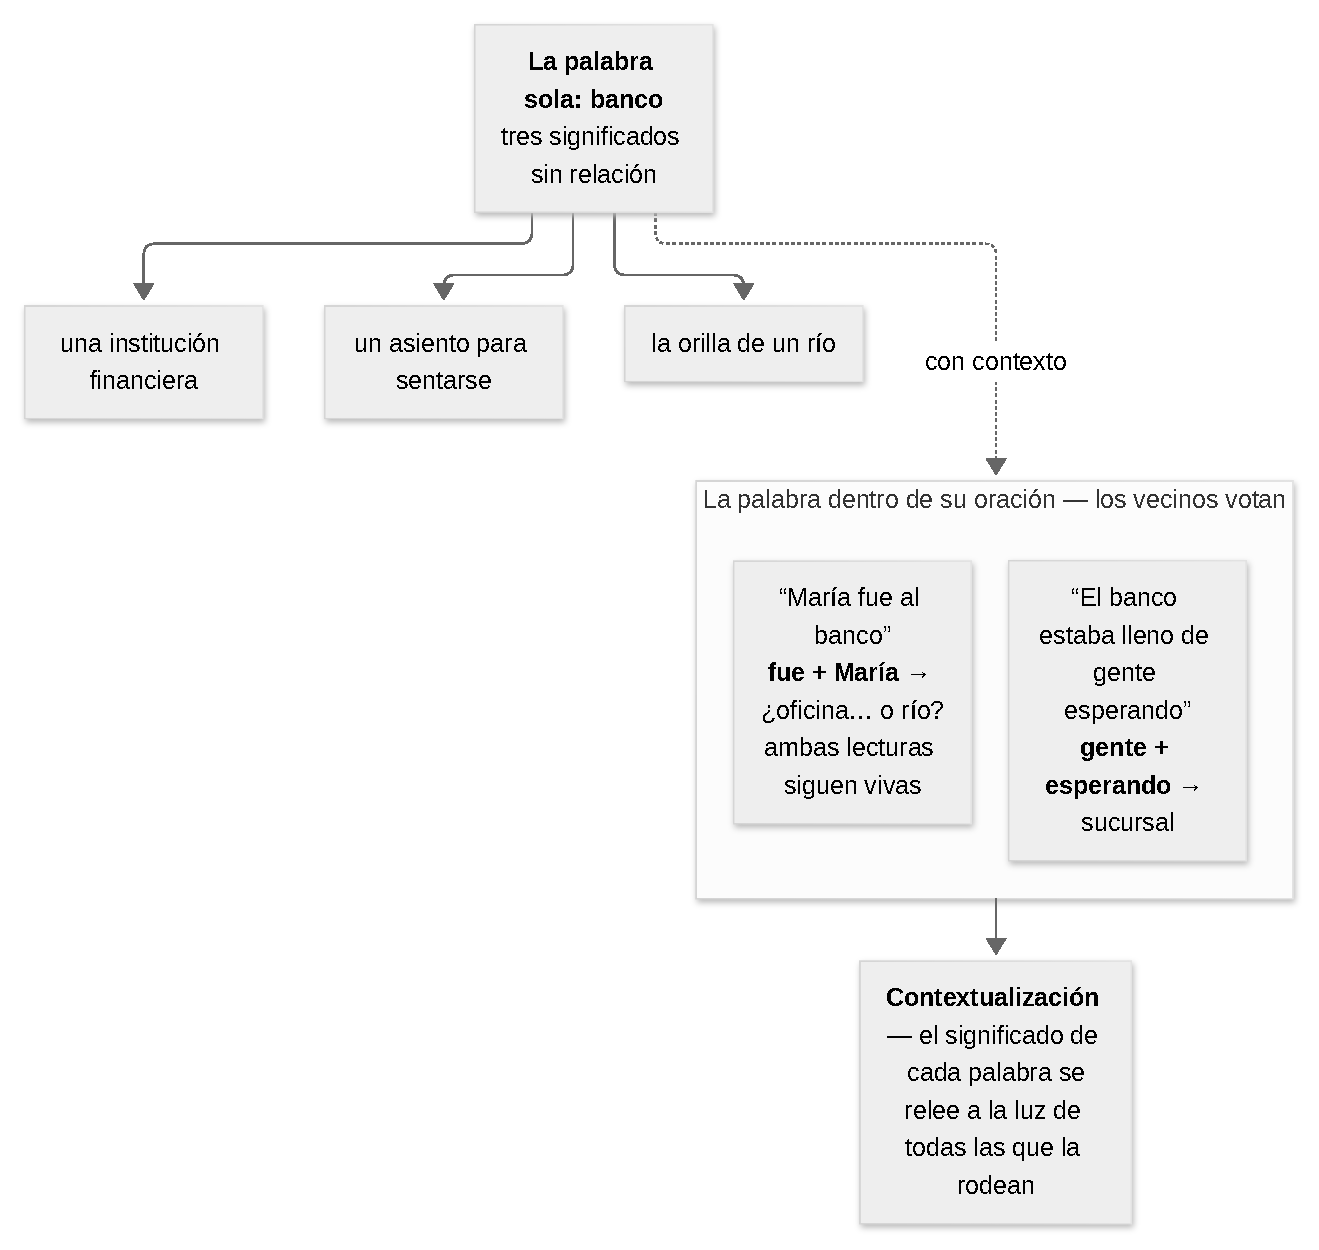
\includegraphics{../paper/figures/tutorial/tutorial-context-es.pdf}}
\caption{La contextualización en una imagen: la palabra ``banco'' sola tiene tres significados sin relación (arriba); dentro de su oración, las palabras vecinas votan y eligen la lectura (en medio). Un transformer hace esto con todas las palabras a la vez.}
\label{fig:tut-context}
\end{figure}

Esta capacidad de releer cada palabra a la luz de toda la oración se llama \emph{contextualización}, y es el corazón de todo transformer moderno. La pregunta que responde este apéndice es \emph{cómo} decide el modelo a qué vecinos escuchar. La respuesta es la atención.

\subsection{El Mecanismo de Atención: Una Voz en una Habitación Ruidosa}
\label{subsec:tut-attention}

La atención es el ``truco mágico'' detrás de la contextualización. Piensa en una conversación en una habitación ruidosa:

\begin{enumerate}[leftmargin=*]
    \item \textbf{Mucho ruido}: varias personas hablan a la vez, pero una te importa.
    \item \textbf{Ignoras al resto}: tu cerebro enfoca automáticamente esa voz y filtra las demás.
    \item \textbf{Entiendes mejor}: al concentrarte, captas cada palabra con claridad.
\end{enumerate}

El mecanismo neuronal funciona igual, con un giro: \emph{cada palabra de la oración es uno de esos escuchas}. Cada palabra ``pregunta'' qué tan importante es cada otra para entenderse, y luego enfoca su atención en las más relevantes. La habitación es la oración, las voces son las palabras y la capacidad de enfocar es la atención. Conserva esta imagen: cada fórmula de abajo es solo la versión aritmética de escuchar selectivamente.

\subsection{Ejemplo Práctico: Las Dos Vidas de ``come''}
\label{subsec:tut-example}

Veamos el mecanismo trabajando sobre una palabra en dos oraciones distintas. Los números son ilustrativos, pero son exactamente el tipo de tabla que un transformer entrenado calcula --- la Figura~\ref{fig:tut-heatmap} muestra ambos casos.

\subsubsection{Contexto 1: ``El gato come pescado''}

Al procesar ``come'', la palabra-oyente pregunta por cada otra voz de la habitación:
\begin{itemize}[leftmargin=*]
    \item ¿Qué tan relevante es ``El''? Poco --- es solo un artículo. \textbf{Atención baja: 5\%}.
    \item ¿Qué tan relevante es ``gato''? Mucha --- es el sujeto, quien come. \textbf{Atención alta: 55\%}.
    \item ¿Y ``come'' mismo? Un poco --- él mismo. \textbf{Atención baja: 5\%}.
    \item ¿Qué tan relevante es ``pescado''? Mucha --- es lo que se come. \textbf{Atención alta: 35\%}.
\end{itemize}
La nueva representación de ``come'' queda dominada por ``gato'' y ``pescado'': una acción, con su sujeto y su objeto.

\subsubsection{Contexto 2: ``El restaurante come los márgenes de beneficio''}

La misma palabra, otra habitación. Ahora los oyentes que importan son otros:
\begin{itemize}[leftmargin=*]
    \item ``restaurante'' (el sujeto): \textbf{30\%}.
    \item ``márgenes'' (lo que se consume): \textbf{30\%}.
    \item ``beneficio'' (lo afectado): \textbf{27\%}.
    \item ``El'', ``los'', ``de'' y ``come'' mismo: el \textbf{13\%} restante.
\end{itemize}

\begin{figure}[H]
\centering
\fitfigure{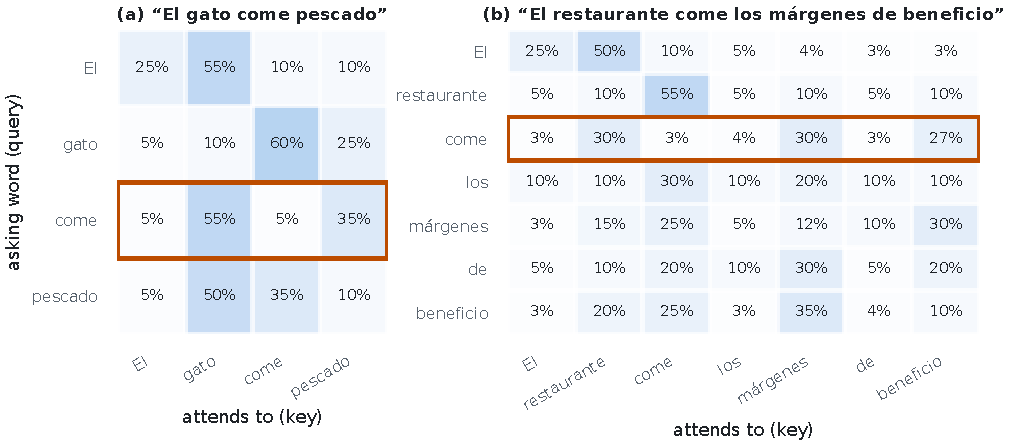
\includegraphics{../paper/figures/tutorial/tut-attention-heatmap-es.pdf}}
\caption{Dos matrices de atención (filas: palabra que pregunta; columnas: palabra escuchada; la fila resaltada es ``come''). En (a) la palabra ``come'' escucha sobre todo a ``gato'' (55\%) y ``pescado'' (35\%); en (b) la misma palabra escucha a ``restaurante'', ``márgenes'' y ``beneficio''. Misma palabra, distinta habitación, distinto enfoque --- la contextualización en acción. Cada fila suma 100\% porque la atención es un presupuesto limitado.}
\label{fig:tut-heatmap}
\end{figure}

La palabra ``come'' termina con una representación completamente distinta en cada oración porque \emph{atiende} a palabras diferentes. Ese es todo el truco: una palabra, muchos significados posibles, y la atención elige a los vecinos correctos para definirla.

\subsection{Cómo Funciona la Atención: Una Biblioteca Llamada Atención}
\label{subsec:tut-math}

Detrás de la escucha hay aritmética. La analogía estándar --- y la que este artículo mantiene --- es una biblioteca, mostrada en la Figura~\ref{fig:tut-qkv}.

\begin{figure}[H]
\centering
\fitfigure{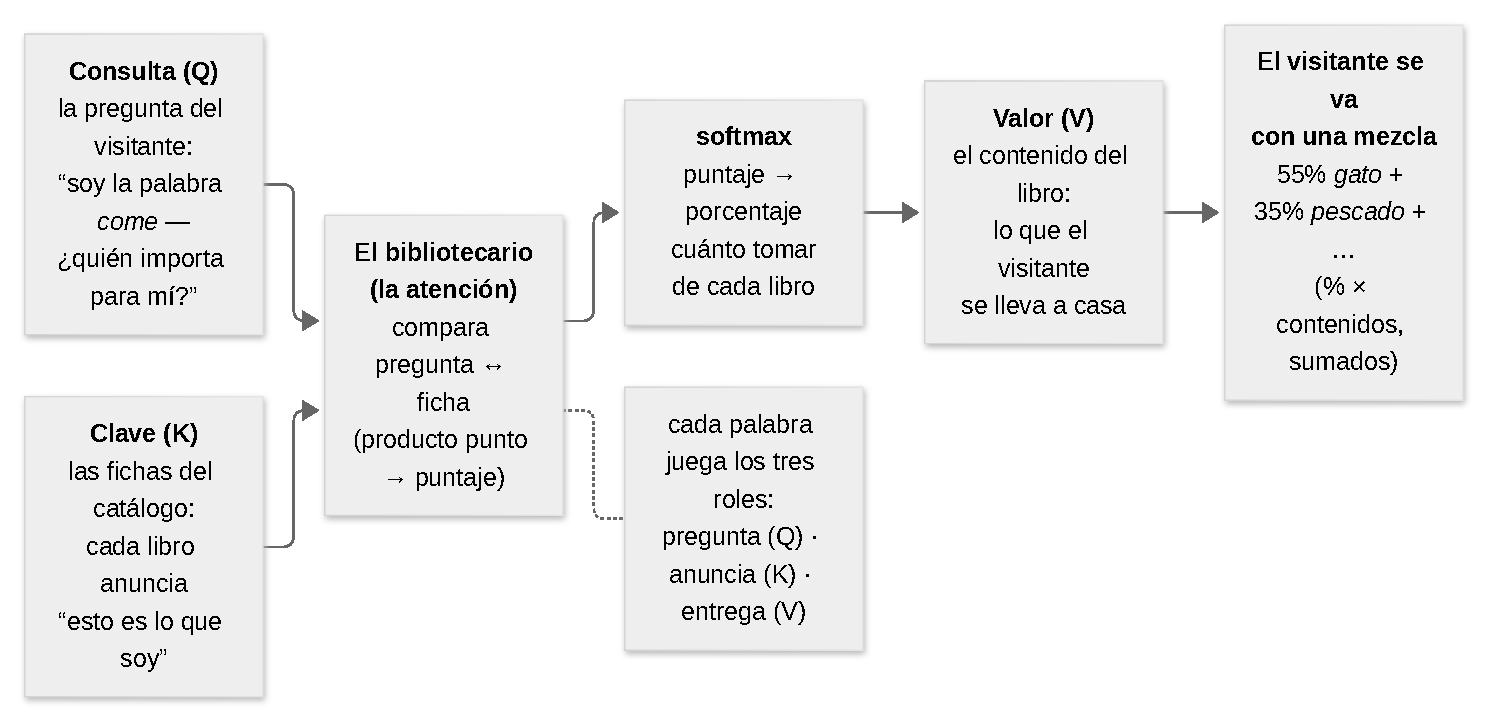
\includegraphics{../paper/figures/tutorial/tutorial-qkv-library-es.pdf}}
\caption{Consultas, claves y valores como una visita a la biblioteca. El visitante lleva una pregunta (Q), cada libro se anuncia con su ficha de catálogo (K), el bibliotecario compara pregunta y fichas (la atención), y el visitante se va con una mezcla ponderada de los contenidos (V).}
\label{fig:tut-qkv}
\end{figure}

\subsubsection{Paso 1: Consultas, Claves y Valores}

Cada palabra se transforma en tres versiones de sí misma:
\begin{itemize}[leftmargin=*]
    \item \textbf{Consulta (Q)}: la pregunta del visitante --- ``¿qué información necesito?''
    \item \textbf{Clave (K)}: la ficha del catálogo --- ``¿qué información ofrezco?''
    \item \textbf{Valor (V)}: el contenido del libro --- ``aquí está mi información real.''
\end{itemize}
Lo crucial: cada palabra juega los tres roles a la vez --- pregunta (Q), se anuncia (K), entrega (V). Una visita a la biblioteca donde cada libro es, al mismo tiempo, visitante y estante.

\subsubsection{Paso 2: Compatibilidad}

El bibliotecario compara la pregunta con cada ficha. Las preguntas parecidas a una ficha obtienen un puntaje alto; el puntaje se calcula multiplicando la consulta por la clave (un \emph{producto punto}). Para nuestra consulta ``come'': $\mathrm{s}(\text{come} \rightarrow \text{gato}) = 3{,}40$, $\mathrm{s}(\text{come} \rightarrow \text{pescado}) = 2{,}95$, $\mathrm{s}(\text{come} \rightarrow \text{El}) = 1{,}00$. La Figura~\ref{fig:tut-attention-steps} reúne los cuatro pasos en un solo cauce.

\begin{figure}[H]
\centering
\fitfigure{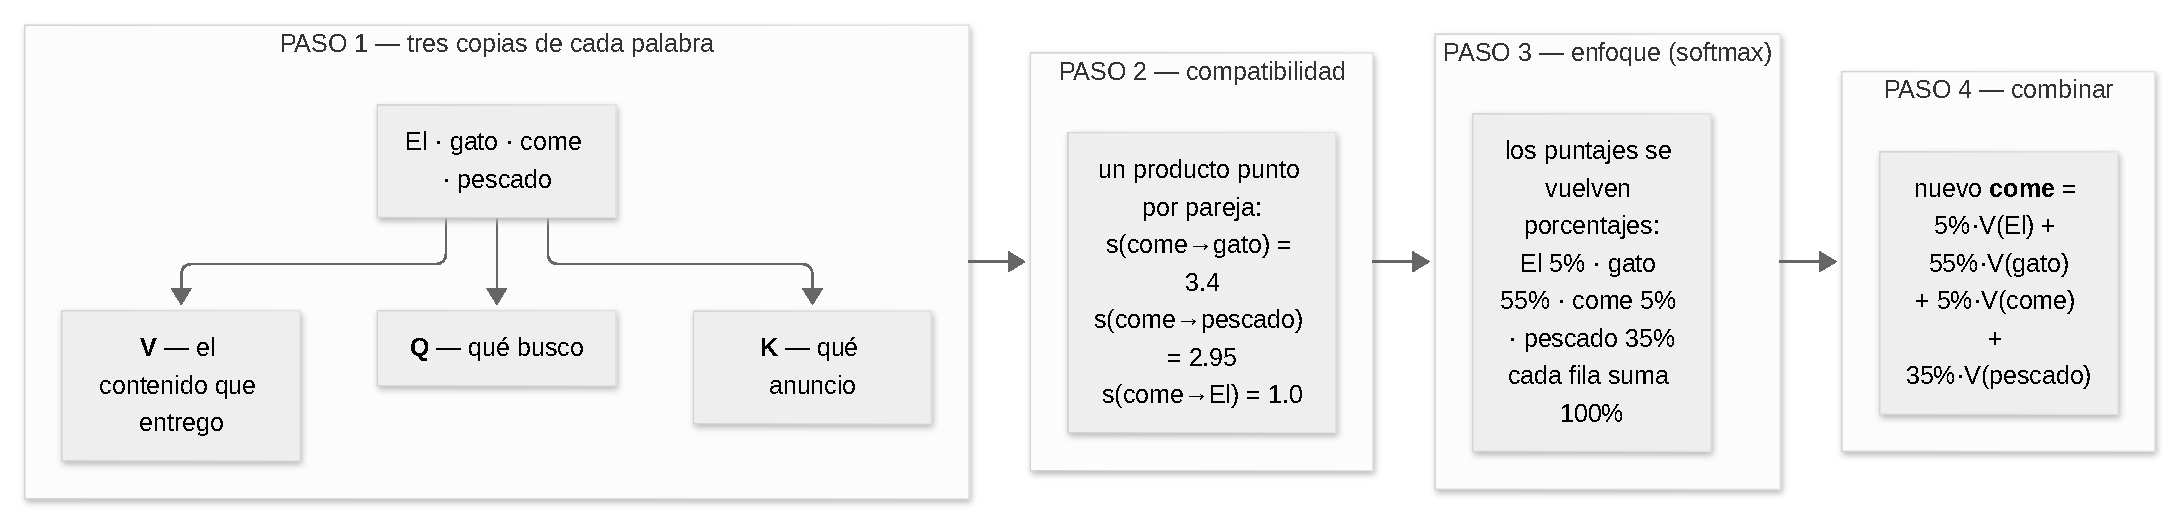
\includegraphics{../paper/figures/tutorial/tutorial-attention-steps-es.pdf}}
\caption{El paso de atención completo para la consulta ``come'' en ``El gato come pescado'': tres copias por palabra (Paso 1), un producto punto por pareja consulta--clave (Paso 2), softmax convirtiendo puntajes en porcentajes (Paso 3) y la combinación ponderada de los valores (Paso 4). Los números son los mismos de las Figuras~\ref{fig:tut-heatmap} y~\ref{fig:tut-softmax}.}
\label{fig:tut-attention-steps}
\end{figure}

\subsubsection{Paso 3: Enfoque}

Los puntajes crudos son solo números; la atención es un \emph{presupuesto}. Una función llamada \texttt{softmax} convierte los puntajes en porcentajes que siempre suman 100\%: la consulta ``come'' convierte los puntajes anteriores en \textbf{5\% / 55\% / 5\% / 35\%} sobre ``El / gato / come / pescado''. La Figura~\ref{fig:tut-softmax} muestra la conversión. Compatibilidad alta significa ``enfoca la atención aquí''; compatibilidad baja significa ``ignora esto'' --- de vuelta en la habitación ruidosa, la voz que decidiste filtrar.

\begin{figure}[H]
\centering
\fitfigure{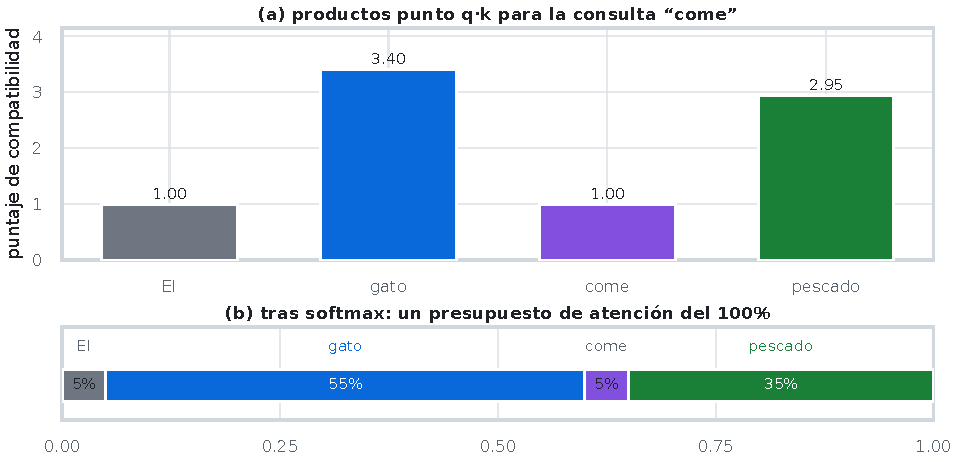
\includegraphics{../paper/figures/tutorial/tut-softmax-focus-es.pdf}}
\caption{Paso 2 $\rightarrow$ Paso 3 en números. Arriba: los cuatro puntajes crudos de compatibilidad (productos punto) para la consulta ``come''. Abajo: tras \texttt{softmax}, los mismos cuatro números se vuelven un presupuesto de atención que suma exactamente 100\%.}
\label{fig:tut-softmax}
\end{figure}

\subsubsection{Paso 4: Combinar}

Finalmente, el visitante se va de la biblioteca con una mezcla ponderada de contenidos. Si ``come'' pone 55\% de su presupuesto en ``gato'' y 35\% en ``pescado'', entonces 55\% del valor de gato y 35\% del valor de pescado se mezclan en la nueva representación de ``come'':
\begin{equation}
\text{nuevo ``come''} \;=\; 5\%\cdot v_{\text{El}} + 55\%\cdot v_{\text{gato}} + 5\%\cdot v_{\text{come}} + 35\%\cdot v_{\text{pescado}}.
\label{eq:tut-mix}
\end{equation}
Ese vector mezclado es lo que ve el resto de la red: una representación de ``come'' que ya contiene quién come y qué se come.

\subsection{Múltiples Cabezas de Atención: Un Equipo de Analistas}
\label{subsec:tut-heads}

Los transformers nunca ejecutan una sola atención sino \emph{muchas cabezas en paralelo} --- como si la oración la analizara un equipo de especialistas, cada uno con una pregunta distinta (Figura~\ref{fig:tut-heads}):

\begin{itemize}[leftmargin=*]
    \item \textbf{Analista 1 (gramática)}: ``¿quién lo hace?'' --- enlaza \emph{gato} $\rightarrow$ \emph{come}.
    \item \textbf{Analista 2 (objeto)}: ``¿qué lo recibe?'' --- enlaza \emph{come} $\rightarrow$ \emph{pescado}.
    \item \textbf{Analista 3 (tiempo)}: ``¿cuándo / con qué frecuencia?'' --- sigue el tiempo verbal y las marcas de tiempo.
    \item \textbf{Analista 4 (estilo)}: ``¿qué artículos y modificadores?'' --- sigue ``el'', ``un'', los adjetivos.
\end{itemize}

\begin{figure}[H]
\centering
\fitfigure{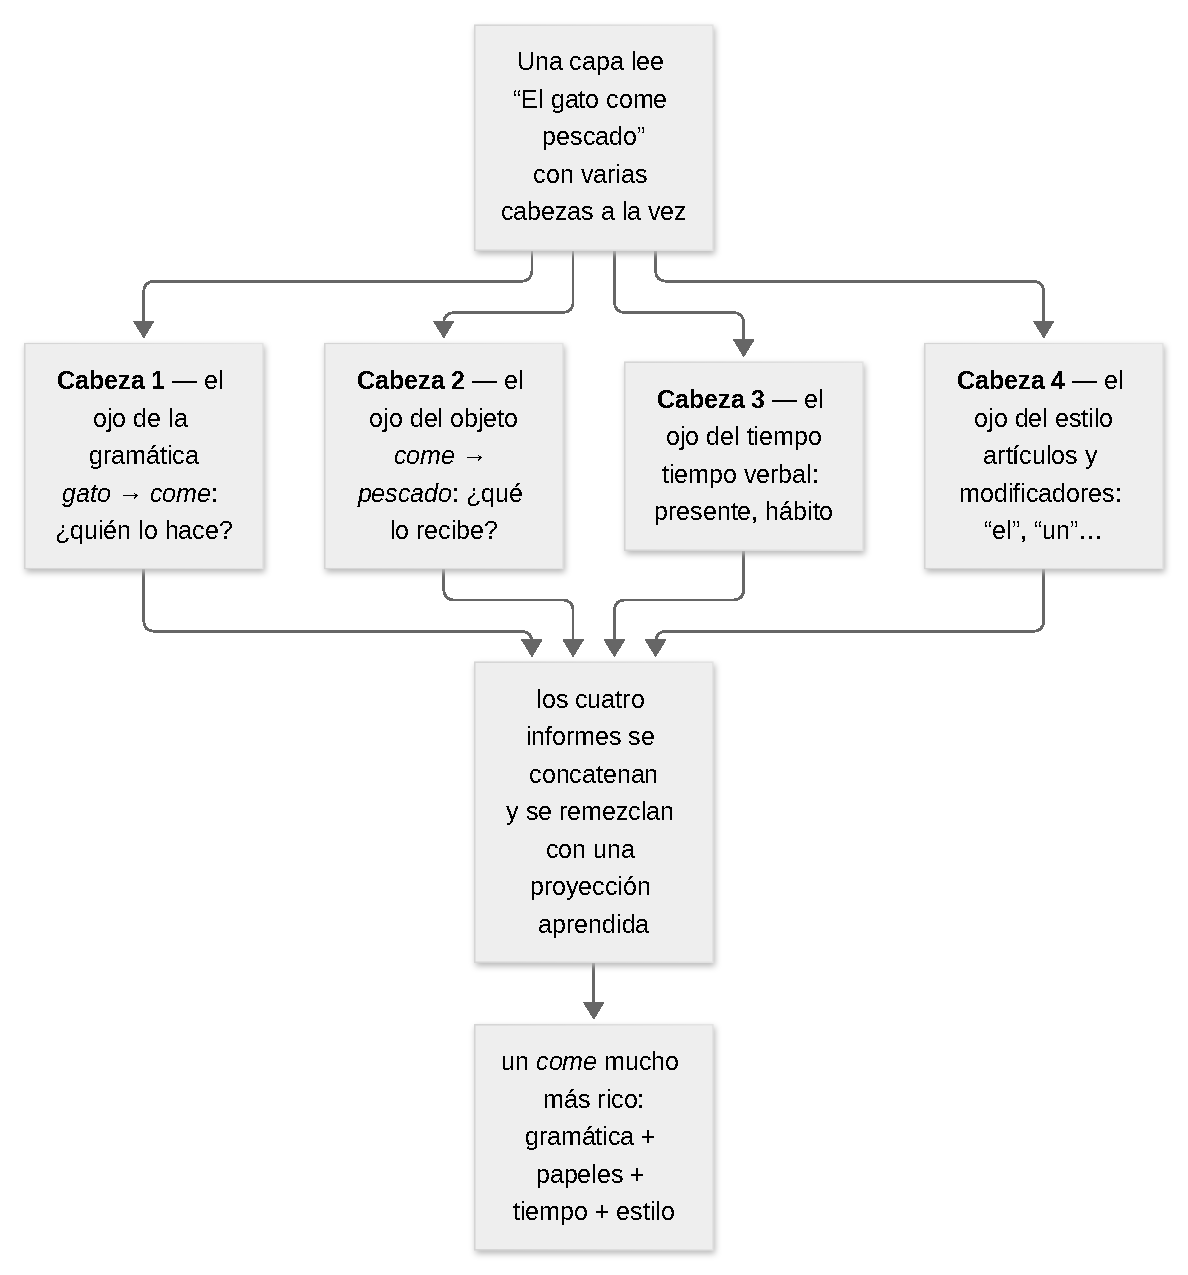
\includegraphics{../paper/figures/tutorial/tutorial-heads-es.pdf}}
\caption{Varias cabezas leen la misma oración simultáneamente, como un equipo de analistas con una pregunta cada una. Sus informes se concatenan y se remezclan en una sola representación mucho más rica.}
\label{fig:tut-heads}
\end{figure}

Cada cabeza aprende su propio patrón de enfoque a partir de los datos, y sus informes se concatenan y remezclan con una proyección aprendida. Juntas capturan mucho más que una sola cabeza --- gramática, papeles, tiempo y estilo a la vez.

\subsection{Apilar Capas: Editar el Ensayo en Pasadas}
\label{subsec:tut-layers}

Un paso de atención todavía ve patrones someros, así que los transformers apilan el mismo bloque muchas veces (de 12 a 48 en modelos prácticos). La analogía: editar un ensayo en pasadas sucesivas (Figura~\ref{fig:tut-layers}).

\begin{enumerate}[leftmargin=*]
    \item \textbf{Primera pasada} --- corregir ortografía y gramática básica: reconocer palabras, formas, género.
    \item \textbf{Segunda pasada} --- aclarar cada oración: quién hace qué y a quién.
    \item \textbf{Tercera pasada} --- asegurar consistencia y flujo narrativo: modismos, relaciones, significado abstracto.
\end{enumerate}

\begin{figure}[H]
\centering
\fitfigure{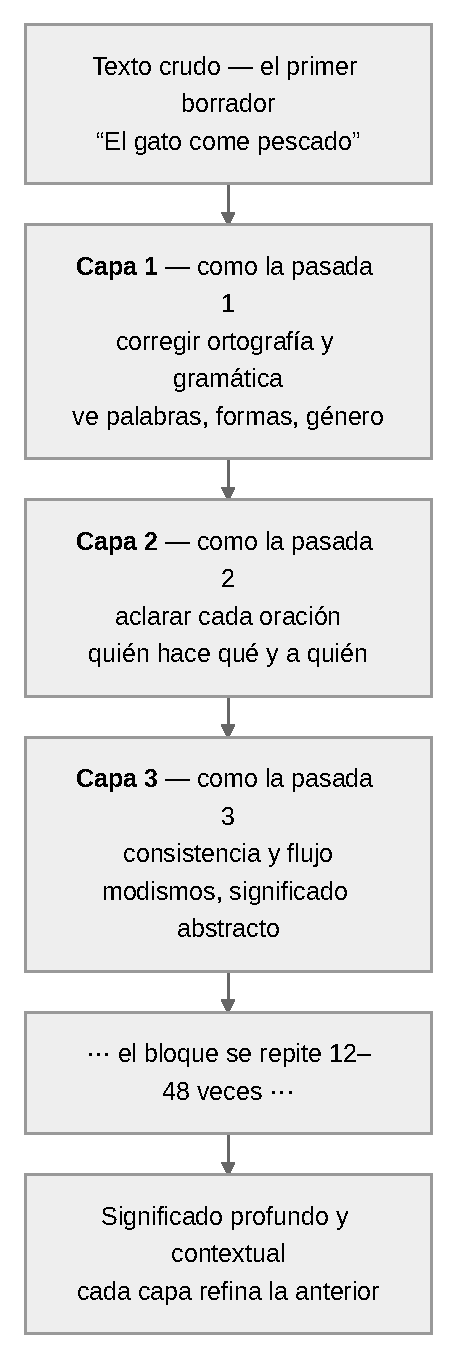
\includegraphics{../paper/figures/tutorial/tutorial-layers-es.pdf}}
\caption{Las capas como pasadas de edición: el texto crudo entra arriba y cada capa refina la lectura de la anterior --- de las palabras y sus formas, pasando por la estructura de la oración, hasta el significado abstracto. El bloque se repite 12--48 veces en la práctica.}
\label{fig:tut-layers}
\end{figure}

Cada capa relee lo que produjo la anterior y lo refina: las primeras capturan características básicas, las posteriores entienden relaciones complejas y conceptos abstractos. Ninguna capa recibe instrucciones sobre qué buscar --- las pasadas se organizan solas durante el entrenamiento.

\subsection{¿Por Qué es Importante?}

El mecanismo de atención fue revolucionario porque:
\begin{enumerate}[leftmargin=*]
    \item \textbf{Paralelismo}: cualquier palabra puede compararse con cualquier otra \emph{a la vez} (sin procesamiento secuencial, a diferencia de los sistemas recurrentes anteriores) --- rápido en hardware moderno.
    \item \textbf{Flexibilidad}: los patrones se aprenden de los datos; nadie programa las reglas.
    \item \textbf{Escalabilidad}: el mismo mecanismo va de una oración a millones de palabras de contexto.
    \item \textbf{Generalidad}: traducción, resumen, preguntas-respuestas, generación, visión por computadora, audio --- un mecanismo, muchas tareas.
\end{enumerate}

\subsection{Desafíos Prácticos: El Precio de Escuchar a Todos}
\label{subsec:tut-challenges}

La atención densa compra su poder comparando \emph{cada} palabra con \emph{todas} las demás, y ese precio crece rápido.

\subsubsection{Complejidad Computacional}

Un documento de 1.000 palabras obliga a $1.000 \times 1.000 = 1.000.000$ de comparaciones palabra a palabra, y el costo se cuadruplica al crecer el documento. La Figura~\ref{fig:tut-complexity} muestra ese crecimiento frente a las alternativas más amables que se comentan abajo.

\begin{figure}[H]
\centering
\fitfigure{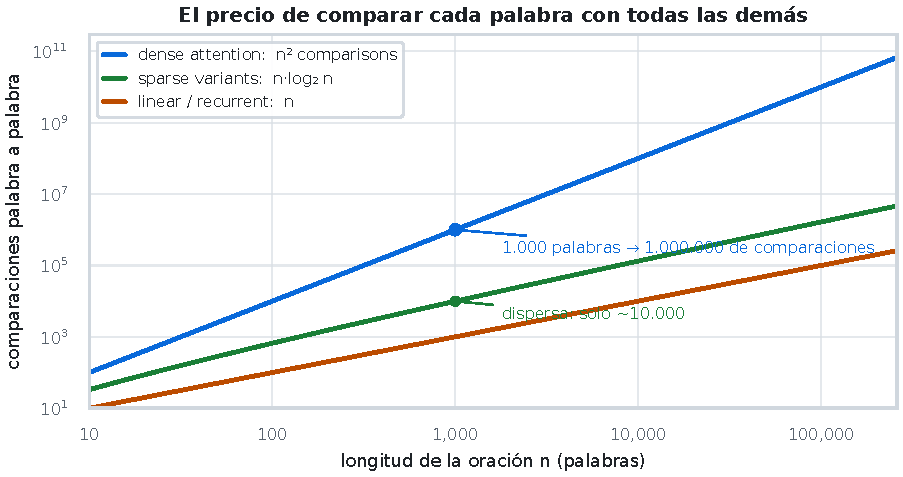
\includegraphics{../paper/figures/tutorial/tut-complexity-growth-es.pdf}}
\caption{Comparaciones palabra a palabra frente a la longitud de la oración. La atención densa compara cada palabra con todas las demás ($n^2$): con $n = 1.000$ ya son un millón de comparaciones. Las variantes dispersas ($n \log_2 n$) y los modelos lineales / recurrentes ($n$) crecen con mucha más suavidad.}
\label{fig:tut-complexity}
\end{figure}

\subsubsection{Requisitos de Memoria}

Durante la inferencia (al usar un modelo entrenado), hay que guardar las claves y valores de cada palabra pasada --- la biblioteca mantiene todos los libros sobre la mesa por si una consulta posterior los necesita. En contextos largos, esa caché domina la memoria de GPU.

\subsubsection{Eficiencia del Dispositivo}

Los transformers se diseñaron para TPUs y GPUs potentes; ejecutarlos en teléfonos o dispositivos integrados es un desafío.

\subsection{Soluciones Modernas: Formas Más Inteligentes de Escuchar}
\label{subsec:tut-solutions}

El resto de este artículo es un catálogo de formas de conservar los beneficios de la atención pagando menos. Cada una conserva nuestras analogías:

\begin{itemize}[leftmargin=*]
    \item \textbf{Atención dispersa}: deja de revisar \emph{cada} ficha de la biblioteca --- visita solo los estantes cercanos y algunos estratégicos. La complejidad baja de $\mathcal{O}(n^2)$ a $\mathcal{O}(n \log n)$ o $\mathcal{O}(n)$.
    \item \textbf{Modelos recurrentes} (p.\ ej.\ Mamba): toma apuntes mientras lees, en vez de reescuchar toda la habitación por cada palabra nueva --- una idea vieja (la recurrencia) reconstruida con eficiencia moderna.
    \item \textbf{Atención con compuerta}: un portero decide qué apuntes valen la pena conservar y cuáles desvanecer, así hay que guardar menos.
    \item \textbf{Cuantización}: escribe cada número con menos dígitos (enteros pequeños en lugar de decimales anchos), reduciendo la memoria con pérdida mínima de precisión.
\end{itemize}

Estas innovaciones son exactamente las que este kit de herramientas (Frankenstein) te permite experimentar, y los apéndices que siguen son recorridos guiados por cada familia.

\subsection{Conclusiones Clave}

\begin{itemize}[leftmargin=*]
    \item Un \textbf{transformer} contextualiza: rele cada palabra a la luz de todos sus vecinos (el ``banco'' ambiguo).
    \item La \textbf{atención} es escucha selectiva: cada palabra reparte su presupuesto limitado del 100\% entre los vecinos que la definen (la habitación ruidosa).
    \item La aritmética es una visita a la biblioteca: la \textbf{consulta} pregunta, la \textbf{clave} se anuncia, el \textbf{valor} entrega; los productos punto puntúan la compatibilidad, \texttt{softmax} convierte puntajes en un presupuesto del 100\%, y los valores se mezclan según ese presupuesto.
    \item Las \textbf{múltiples cabezas} son un equipo de analistas con una pregunta cada una; las \textbf{capas apiladas} son pasadas de edición sucesivas, cada una refinando la anterior.
    \item El problema: la atención densa compara a todos con todos --- $\mathcal{O}(n^2)$ --- y por eso existen las variantes dispersas, recurrentes, con compuerta y cuantizadas.
    \item Cada apéndice posterior es un recorrido más profundo por una de esas variantes; las analogías de la Tabla~\ref{tab:tut-analogies} seguirán volviendo.
\end{itemize}
